\section{Datenbank Modelle}
In diesem Abschnitt werden die Grundlagen, der relationalen und Graph basierten Datenbank-Modell skizziert. Diese sind im Rahmen dieser Arbeit von wesentlicher Bedeutung. Schließlich vereint die in \compref{chap:db2graph} beschriebene Graph-Erweiterung sowohl Elemente des relationalen, als auch des Graph-Modells.

Um einen Überblick über die beiden Modelle zu geben, werden beide unter einem jeweiligen Aspekt des Modells einander gegenüber gestellt. Zu den Aspekten dieses Vergleichs gehören: 

\begin{itemize}
    \item Herkunft \& Verbreitung,
    \item Struktur \& Schema,
    \item Beziehungen und
    \item Abfragesprachen.
\end{itemize}

Die Beschränkung auf diese Aspekte wurde dabei vorgenommen, da ein tiefgreifender Vergleich beider Modelle über den Rahmen der Arbeit hinausgehen würde. Ziel dieses Abschnitts ist es lediglich einen kleinen Überblick über die verschiedenen Modelle zu geben. 

\subsection{Herkunft \& Verbreitung}
In diesem Unterabschnitt wird auf die Herkunft und aktuelle Verbreitung der beiden Modell eingegangen. Die Verbreitung wird dabei an der aktuellen Verbreitung von relationalen und Graph-Datenbanksystemen gemessen. 

\subsubsection{Relationales Modell}
Das relationale Modell hat seinen Ursprung in den 1970er Jahren \cite{rdbms_history}. Seine Grundlagen wurden dabei erstmals in \cite{codd_relational_model} von \citeauthor{codd_relational_model} umrissen. In den folgenden Jahren  wurde beim IBM Research unter dem Namen \textit{System R} ein erstes relationales Datenbanksystem entwickelt \cite{rdbms_history}. Es gilt dabei herauszustellen, dass die Paper die im Zuge der Forschung und Entwicklung am \textit{System R} veröffentlicht wurden, der Öffentlichkeit frei zur Verfügung gestellt wurden \cite{rdbms_history}. 

Heute haben relationale Datenbanksysteme eine große Verbreitung gefunden, siehe \autoref{}. So sollen nach \cite{db_engines_ranking_july} relationale Datenbanksysteme 72,7 \% des gesamten Datenbankmarktes ausmachen (Stand Juli 2021). Folglich kann dem relationalen Modell und relationalen Datenbanksystemen eine marktbeherrschende Rolle zugeschrieben werden.

% TODO INSERT PIE CHART

\subsubsection{Graph-Modell}
Das Graph- als Datenbank-Modell hat seinen Ursprung in der heutigen Form im Jahr 1999 \cite{gdbms}. Dabei wurde das Graph-Modell mit der Motivation entwickelt, vermeintliche Nachteile oder Probleme des relational Modells auszuräumen \cite{gdbms}.

Graphdatenbanksysteme und das Graph-Modell sind heute als vergleichbar junge Technologien sind heute noch nicht so weit verbreitet, wie beispielsweise, dass relationale Modell. Mit 1,7 \% Marktanteil ordnen sich Graph-Datenbanksysteme, noch weit hinter anderen Technologien ein, wie \textit{Document Stores}, \textit{Key-Values Stores} oder \textit{Wide column stores} \cite{db_engines_ranking_july}, siehe \autoref{}. Jedoch haben Graphdatenbanksysteme seit 2013 einen erheblichen Aufschwung in Popularität erfahren \cite{db_engines_ranking_july}. 

\subsection{Struktur \& Schema}
\label{datenmodelle:structure}
Im Rahmen dieses Abschnitts wird auf die vorhandenen Strukturen der Datenbankmodelle eingegangen. Darüber hinaus wird auch das zugrundeliegende Schema genauer erläutert. 

\subsubsection{Relationales Modell}
\label{datenmodelle:structure:relational}
Im Zentrum des relationalen Modells steht hierbei das sogenannte Informationsprinzip \cite{rdbms_history}. Dies beschreibt, dass alle Informationen in einer Datenbank ausschließlich in exakt einer Weise repräsentiert werden dürfen \cite{codd_relational_model}. Informationen werden dabei in Form von Tupeln und Relationen organisiert \cite{codd_relational_model}. Für deren Organisation stellen relationale Datenbanksysteme Tabellen, Spalten und Zeilen als Strukturen bereit \cite{rdbms_history}. So werden auf Basis des Informationsprinzips, alle Informationen als Werte in einer Zelle einer bestimmten Tabelle abgelegt \cite{rdbms_history}. So lassen sich beispielsweise alle Entitäte  vom Entitätstyp Auto in einer relationalen Tabelle abbilden, siehe \autoref{tab:auto_tabelle}. 

\begin{table}[h]
    \centering
    \begin{tabular}{c|c|c|c}
    \hline
    \rowcolor[HTML]{EFEFEF} 
    \multicolumn{1}{l|}{\cellcolor[HTML]{EFEFEF}\textbf{Fahrzeugnummer}} & \multicolumn{1}{l|}{\cellcolor[HTML]{EFEFEF}\textbf{Marke}} & \multicolumn{1}{l|}{\cellcolor[HTML]{EFEFEF}\textbf{Model}} & \multicolumn{1}{l}{\cellcolor[HTML]{EFEFEF}\textbf{Baujahr}} \\ \hline
    FZ-123456789 & Toyota & Starlet & 1997 \\
    FZ-234567890 & Nissan & Leaf & 2018 \\
    FZ-345678912 & VW & ID3 & 2020 \\
    FZ-456789123 & Ford & Fiesta & 2001 \\
    ... & ... & ... & ... \\ \hline
    \end{tabular}
    \caption{Beispiel relationale Tabelle für den Entitätstyp Auto}
    \label{tab:auto_tabelle}
\end{table}

Das relationale Modell setzt bei der Datenhaltung allerdings ein striktes Schema voraus \cite{rdbms_book}. Schließlich fordert das Informationsprinzip, dass alle Informationen immer in genau einer Art und Weise repräsentiert werden müssen \cite{rdbms_history}. Es verlangt somit eine homogene Darstellung der Daten. Allerdings sind viele Daten in der realen Welt heterogen. Dies hat zu Folge, dass Daten einen sogenannten Normalisierungsprozess durchlaufen müssen \cite{rdbms_book}. Bei diesem Prozess werden die Daten in die sogenannte dritte Normalform (3NF) gebracht, wodurch jegliche Anomalien vermieden werden können \cite{rdbms_book}. So können letztendlich die Informationen einer Entität in einem homogenen Typschema abgebildet werden. 

\subsubsection{Graph-Modell}
Die Grundlage des Graph-Modells stellen sogenannte Vertexes und Edges dar, auf Deutsch Knoten und Kanten \cite{gdbms}. Diese Vertexes und Edges bilden dabei zusammen einen sogenannten Graphen. So werden in einem Graphen einerseits Entitäten in Form eines Knotens repräsentiert \cite{gdbms}. Anderseits bildet es auch explizit Beziehungen zwischen Entitäten mittels Kanten ab \cite{gdbms}. Darauf wird aber \autoref{datenmodelle:beziehungen}  weiter eingegangen.

Das Graph-Modell setzt im Gegensatz zum relationalen Modell auf ein flexibles Datenschema \cite{gdbms}. Dadruch unterstützt es den Umgang mit heterogenen Daten \cite{gdbms}. Denn anstatt einer strikten Typisierung der Entitäten -- durch Tabellen im relationalen Modell -- lassen sich die Daten im Graph-Modell anhand von Labels organisiert werden. Labels markieren dabei Knoten oder Kanten, die dieselbe oder eine ähnliche Rolle einnehmen. Sie sind in ihrer Funktion allerdings nicht mit Tabellen aus dem relationalen Modell vergleichbar. Dies liegt darin begründet, dass Entitäten mit einem bestimmten Label unterschiedliche Informationen aufweisen können. 

\subsection{Beziehungen}
\label{datenmodelle:beziehungen}
In diesem Abschnitt wird darauf eingegangen, wie und in welcher Form die Modelle mit Beziehungen zwischen Entitäten abbilden. 

\subsubsection{Relationales Modell}
Das relationale Modell unterstützt Beziehungen insofern, dass es möglich ist Beziehungen zwischen Entitätstyp zu definieren. Diese Beziehungen dabei lassen sich in die drei folgenden Kategorien unterteilen: 
\begin{itemize}
    \item \textit{one-to-one}, 
    \item \textit{one-to-many} (beziehungsweise \textit{many-to-one}) und 
    \item \textit{many-to-many}.
\end{itemize}

Bei der Repräsentation aller Beziehungskategorien spielen  folgenden Begriffe eine Schlüsselrolle:
\begin{itemize}
    \item \textit{Primärschlüssel}\\
    Beschreibt das Einzigartigkeitskriterium der Zeilen in einer Tabelle. Kann sich dabei auch aus mehreren Spalten zusammensetzen. 
    \item \textit{Sekundärschlüssel}\\
    Referenziert Zeilen einer anderen Tabelle B anhand des dortigen Primärschlüssels. Er gibt dabei an, welche Spalten von Tabelle A zur Referenz des Primärschlüssels genutzt werden. 
    \item \textit{Joins}\\
    Ermöglichen es solche Referenzen im Kontext einer Abfrage aufzulösen.
\end{itemize}

Bei \textit{one-to-one}- oder \textit{many-to-one}-Beziehungen ist es hierbei ausreichen, den oder die anderen Zeilen aus einer Tabelle mittels Sekundärschlüssel und Primärschlüssels zu referenzieren. Sollten die Informationen dann abgefragt werden, kann die Referenzierung durch einen Join aufgelöst werden.

Das Abbilden von \textit{many-to-many}-Beziehungen erfordert hingegen die Einführung einer Auflösungstabelle, siehe die Kfz-Register Tabelle in \autoref{fig:relationales_modell_many-to-many}. 

\begin{figure}[h]
    \centering
    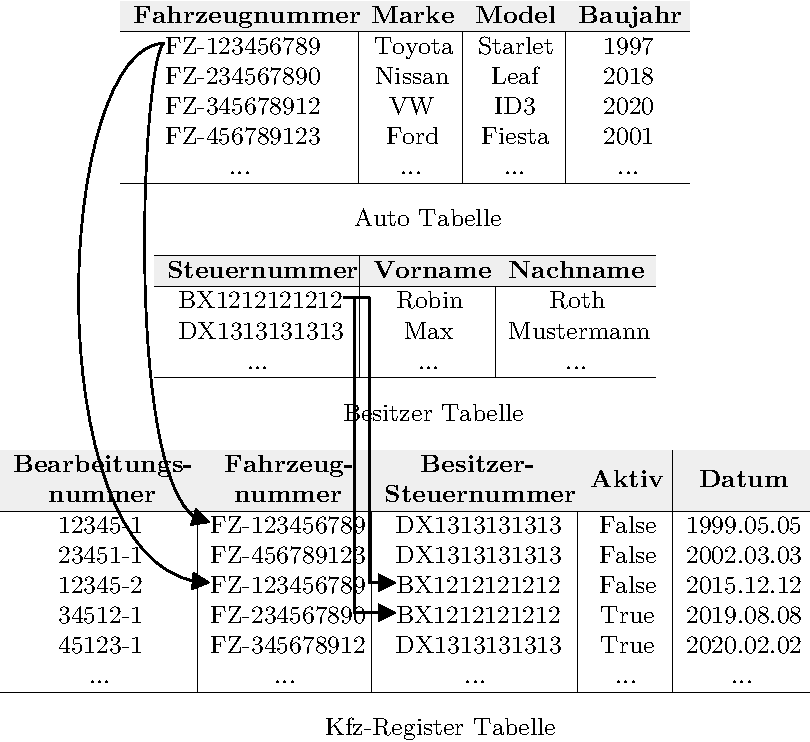
\includegraphics[width=\textwidth]{images/many-to-many.pdf}
    \caption{Beispiel many-to-many-Beziehungen im relationalen Modell}
    \label{fig:relationales_modell_many-to-many}
\end{figure}

\subsubsection{Graph-Modell}
Beim Graph-Modell stellen Beziehungen eine grundlegende Struktur in einem Graphen dar, siehe \autoref{datenmodelle:structure}. Dabei werden im Graph-Modell Beziehungen direkt zwischen Entität aufgebaut, keine Entitätstypen wie im relationalen Modell. 

Es unterstützt dabei alle drei Beziehungskategorien die aus dem relationalen Modell bekannt sind \textit{one-to-one}, \textit{many-to-one} und \textit{many-to-many}. Dabei findet im Graph-Modell keinerlei Unterscheidung zwischen den drei Kategorien statt. Denn zwei Knoten können mehrere Edges haben, die sie miteinander verbinden. Dies ändert aber nichts an Art der Haltung oder Referenzierung von Informationen. Alle Beziehungen werden also immer in Form einer Kante zwischen einem Start- und Zielknoten repräsentiert. Dabei muss allerdings darauf hingewiesen werden, dass der Start- und Zielknoten einer Kante derselbe Knoten sein können.

\subsection{Abfragesprachen}
Im Rahmen dieses Unterabschnitts wird auf Abfragesprachen eingegangen. Dabei werden die Abfragesprachen aufgeführt, die in Datenbanksystemen mit dem jeweiligen Datenmodell verbreitet sind.

\subsubsection{Relationales Modell}
Im Feld der relationalen Datenbanksysteme ist die Abfragesprache SQL weit verbreitet \cite{sql_history}. Sie wurde von Donald D. Chamberlin und Raymond F. Boyce im Rahmen des \textit{System R} Projekts entwickelt \cite{sql_history}. SQL wurde dabei mit der Motivation entworfen eine einfache Abfragesprache für relationale Daten zu entwickeln \cite{sql_history}. 

Bei SQL handelt es sich um eine deklarative Abfragesprache \cite{sql_history}. Der grundlegende Aufbau der Sprache und die Syntax können dabei der \autoref{src:sql_example} entnommen werden. So ist in \autoref{src:sql_example} klar erkennbar, dass sich alle Operationen auf Tabellen und Spalten beziehen. So arbeitet die Sprache -- wie erwartet -- in den Strukturen des relationalen Modells.

\begin{lstlisting}[caption={Beispiel SQL-Queries},language=SQL,label=src:sql_example]
/* Tabelle erstellen */
CREATE TABLE Autos (
    Fahrzeugnummer VARCHAR(50), 
    Marke VARCHAR(10), 
    Modell VARCHAR(10), 
    Baujahr INT,
    Primary Key(Fahrzeugnummer)
);

/* Daten in Tabelle schreiben */
INSERT INTO Autos 
(Fahrzeugnummer, Marke, Modell, Baujahr) 
("FZ-123456789", "Toyota", "Starlet", 1997);

/* Daten Abfragen */
SELECT Marke, Model, Baujahr FROM Autos 
WHERE Fahrzeugnummer = "FZ-123456789";

/* Daten Loeschen */
DELETE FROM Autos WHERE Fahrzeugnummer = "FZ-123456789";
\end{lstlisting}

Des Weiteren muss darauf hingewiesen werden, dass SQL als Sprache standardisiert wurde \cite{sql_history}. Allerdings gibt es heute trotz des Standards weiterhin sogenannte SQL-Dialekte. So können sich einige SQL Sprachelemente je nach Datenbanksystem oder Hersteller weiterhin unterscheiden. 

\subsubsection{Graph-Modell}

